\begin{figure*}[t]
\centering
\definecolor{uvcfive}{HTML}{999999}
\definecolor{uvcsixteen}{HTML}{0072B2}
\definecolor{d435line}{HTML}{0072B2}
\definecolor{d455line}{HTML}{D55E00}
\resizebox{\linewidth}{!}{%
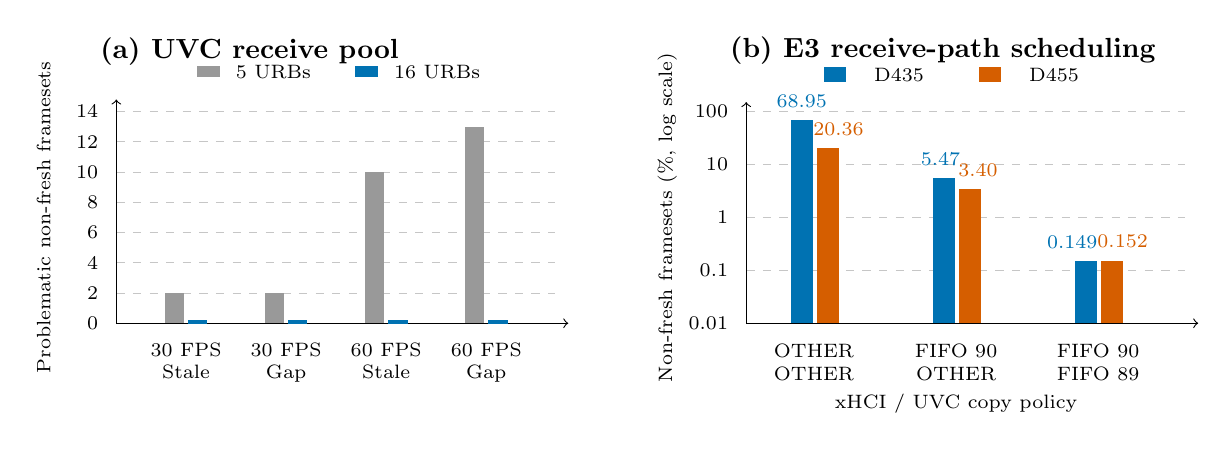
\begin{tikzpicture}[font=\scriptsize]
  % (a) UVC receive-pool freshness failures.
  \begin{scope}[x=0.82cm,y=0.192cm]
    \node[anchor=west,font=\bfseries] at (0.55,18.0) {(a) UVC receive pool};
    \fill[uvcfive] (2.20,16.3) rectangle (2.55,17.0);
    \node[anchor=west] at (2.65,16.65) {5 URBs};
    \fill[uvcsixteen] (4.65,16.3) rectangle (5.00,17.0);
    \node[anchor=west] at (5.10,16.65) {16 URBs};
    \foreach \v in {0,2,...,14} {
      \draw[gray!45,dashed,line width=0.25pt] (0.95,\v) -- (7.75,\v);
      \node[anchor=east] at (0.82,\v) {\v};
    }
    \draw[->] (0.95,0) -- (7.95,0);
    \draw[->] (0.95,0) -- (0.95,14.8);
    \node[rotate=90,anchor=south,font=\scriptsize] at (0.08,7.0) {Problematic non-fresh framesets};

    \fill[uvcfive] (1.70,0) rectangle (2.00,2);
    \fill[uvcfive] (3.25,0) rectangle (3.55,2);
    \fill[uvcfive] (4.80,0) rectangle (5.10,10);
    \fill[uvcfive] (6.35,0) rectangle (6.65,13);
    \draw[uvcsixteen,line width=1.4pt] (2.06,0.08) -- (2.36,0.08);
    \draw[uvcsixteen,line width=1.4pt] (3.61,0.08) -- (3.91,0.08);
    \draw[uvcsixteen,line width=1.4pt] (5.16,0.08) -- (5.46,0.08);
    \draw[uvcsixteen,line width=1.4pt] (6.71,0.08) -- (7.01,0.08);
    \node[align=center,anchor=north] at (2.03,-0.65) {30 FPS\\Stale};
    \node[align=center,anchor=north] at (3.58,-0.65) {30 FPS\\Gap};
    \node[align=center,anchor=north] at (5.13,-0.65) {60 FPS\\Stale};
    \node[align=center,anchor=north] at (6.68,-0.65) {60 FPS\\Gap};
  \end{scope}

  % (b) E3 non-fresh framesets under progressive kernel-path protection.
  \begin{scope}[xshift=8.0cm,x=0.82cm,y=0.672cm]
    \node[anchor=west,font=\bfseries] at (0.55,5.15)
      {(b) E3 receive-path scheduling};
    \fill[d435line] (2.15,4.55) rectangle (2.50,4.85);
    \node[anchor=west] at (2.78,4.70) {D435};
    \fill[d455line] (4.55,4.55) rectangle (4.90,4.85);
    \node[anchor=west] at (5.18,4.70) {D455};
    \foreach \v/\lab in {0/{0.01},1/{0.1},2/{1},3/{10},4/{100}} {
      \draw[gray!45,dashed,line width=0.25pt] (0.95,\v) -- (7.75,\v);
      \node[anchor=east] at (0.82,\v) {\lab};
    }
    \draw[->] (0.95,0) -- (7.95,0);
    \draw[->] (0.95,0) -- (0.95,4.18);
    \node[rotate=90,anchor=south,font=\scriptsize] at (0.03,2.0)
      {Non-fresh framesets (\%, log scale)};

    \fill[d435line] (1.64,0) rectangle (1.98,3.839);
    \fill[d455line] (2.04,0) rectangle (2.38,3.309);
    \fill[d435line] (3.84,0) rectangle (4.18,2.738);
    \fill[d455line] (4.24,0) rectangle (4.58,2.532);
    \fill[d435line] (6.04,0) rectangle (6.38,1.174);
    \fill[d455line] (6.44,0) rectangle (6.78,1.183);
    \node[text=d435line,anchor=south,font=\scriptsize] at (1.81,3.89) {68.95};
    \node[text=d455line,anchor=south,font=\scriptsize] at (2.38,3.36) {20.36};
    \node[text=d435line,anchor=south,font=\scriptsize] at (3.96,2.79) {5.47};
    \node[text=d455line,anchor=south,font=\scriptsize] at (4.54,2.58) {3.40};
    \node[text=d435line,anchor=south,font=\scriptsize] at (6.00,1.23) {0.149};
    \node[text=d455line,anchor=south,font=\scriptsize] at (6.78,1.24) {0.152};
    \node[align=center,anchor=north] at (2.00,-0.22) {OTHER\\OTHER};
    \node[align=center,anchor=north] at (4.20,-0.22) {FIFO 90\\OTHER};
    \node[align=center,anchor=north] at (6.40,-0.22) {FIFO 90\\FIFO 89};
    \node[anchor=north,font=\scriptsize] at (4.20,-1.15) {xHCI / UVC copy policy};
  \end{scope}
\end{tikzpicture}
}
\caption{Host-path controls with frame-acquisition workers under FIFO-RM.
  (a) E2 counts of partially stale framesets and deliveries containing a
stream sequence gap for one D435 with four OTHER CPU competitors.
Each return is counted once in its category.  (b) E3 percentage of
non-fresh framesets---partially or fully stale, affected by a sequence gap, or both---under
targeted CPU~3 starvation and progressive xHCI/UVC copy protection; each
treatment label gives the xHCI IRQ policy above the UVC-copy kworker policy.
Each bar pools three 30-s non-RT \texttt{threadirqs} stress runs.}
\label{fig:linux-host-path-results}
\end{figure*}
